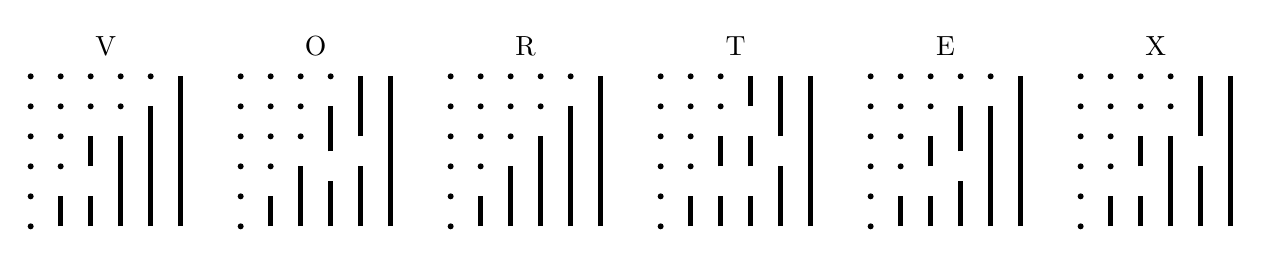
\begin{tikzpicture}[x=0.15in,y=0.15in]
\begin{scope}[shift={(14,0)}]
\fill[white] (0,0) rectangle (5,5);
\foreach \y in {0,1,2,3,4,5} {\fill (0,\y) circle (0.1);}
\foreach \y in {2,3,4,5} {\fill (1,\y) circle (0.1);}
\foreach \y in {3,4,5} {\fill (2,\y) circle (0.1);}
\foreach \y in {4,5} {\fill (3,\y) circle (0.1);}
\foreach \y in {5} {\fill (4,\y) circle (0.1);}
\draw[line width=2pt] (1,0) -- (1,1); 
\draw[line width=2pt] (2,0) -- (2,2); 
\draw[line width=2pt] (3,0) -- (3,3); 
\draw[line width=2pt] (4,0) -- (4,4); 
\draw[line width=2pt] (5,0) -- (5,5); 
\node at (2.5,6) {R};
\end{scope} 
\begin{scope}[shift={(7,0)}]
\fill[white] (0,0) rectangle (5,5);
\foreach \y in {0,1,2,3,4,5} {\fill (0,\y) circle (0.1);}
\foreach \y in {2,3,4,5} {\fill (1,\y) circle (0.1);}
\foreach \y in {3,4,5} {\fill (2,\y) circle (0.1);}
\foreach \y in {5} {\fill (3,\y) circle (0.1);}
\draw[line width=2pt] (1,0) -- (1,1); 
\draw[line width=2pt] (2,0) -- (2,2); 
\draw[line width=2pt] (3,0) -- (3,1.5); \draw[line width=2pt] (3,2.5) -- (3,4); 
\draw[line width=2pt] (4,0) -- (4,2); \draw[line width=2pt] (4,3) -- (4,5); 
\draw[line width=2pt] (5,0) -- (5,5); 
\node at (2.5,6) {O};
\end{scope} 
\begin{scope}[shift={(0,0)}]
\fill[white] (0,0) rectangle (5,5);
\foreach \y in {0,1,2,3,4,5} {\fill (0,\y) circle (0.1);}
\foreach \y in {2,3,4,5} {\fill (1,\y) circle (0.1);}
\foreach \y in {4,5} {\fill (2,\y) circle (0.1);}
\foreach \y in {4,5} {\fill (3,\y) circle (0.1);}
\foreach \y in {5} {\fill (4,\y) circle (0.1);}
\draw[line width=2pt] (1,0) -- (1,1); 
\draw[line width=2pt] (2,0) -- (2,1); \draw[line width=2pt] (2,2) -- (2,3); 
\draw[line width=2pt] (3,0) -- (3,3);
\draw[line width=2pt] (4,0) -- (4,4);
\draw[line width=2pt] (5,0) -- (5,5); 
\node at (2.5,6) {V};
\end{scope} 
\begin{scope}[shift={(35,0)}]
\fill[white] (0,0) rectangle (5,5);
\foreach \y in {0,1,2,3,4,5} {\fill (0,\y) circle (0.1);}
\foreach \y in {2,3,4,5} {\fill (1,\y) circle (0.1);}
\foreach \y in {4,5} {\fill (2,\y) circle (0.1);}
\foreach \y in {4,5} {\fill (3,\y) circle (0.1);}
\draw[line width=2pt] (1,0) -- (1,1); 
\draw[line width=2pt] (2,0) -- (2,1); \draw[line width=2pt] (2,2) -- (2,3); 
\draw[line width=2pt] (3,0) -- (3,3);
\draw[line width=2pt] (4,0) -- (4,2); \draw[line width=2pt] (4,3) -- (4,5); 
\draw[line width=2pt] (5,0) -- (5,5); 
\node at (2.5,6) {X};
\end{scope} 
\begin{scope}[shift={(28,0)}]
\fill[white] (0,0) rectangle (5,5);
\foreach \y in {0,1,2,3,4,5} {\fill (0,\y) circle (0.1);}
\foreach \y in {2,3,4,5} {\fill (1,\y) circle (0.1);}
\foreach \y in {4,5} {\fill (2,\y) circle (0.1);}
\foreach \y in {5} {\fill (3,\y) circle (0.1);}
\foreach \y in {5} {\fill (4,\y) circle (0.1);}
\draw[line width=2pt] (1,0) -- (1,1); 
\draw[line width=2pt] (2,0) -- (2,1); \draw[line width=2pt] (2,2) -- (2,3); 
\draw[line width=2pt] (3,0) -- (3,1.5); \draw[line width=2pt] (3,2.5) -- (3,4);
\draw[line width=2pt] (4,0) -- (4,4);
\draw[line width=2pt] (5,0) -- (5,5); 
\node at (2.5,6) {E};
\end{scope} 
\begin{scope}[shift={(21,0)}]
\fill[white] (0,0) rectangle (5,5);
\foreach \y in {0,1,2,3,4,5} {\fill (0,\y) circle (0.1);}
\foreach \y in {2,3,4,5} {\fill (1,\y) circle (0.1);}
\foreach \y in {4,5} {\fill (2,\y) circle (0.1);}
\draw[line width=2pt] (1,0) -- (1,1); 
\draw[line width=2pt] (2,0) -- (2,1); \draw[line width=2pt] (2,2) -- (2,3); 
\draw[line width=2pt] (3,0) -- (3,1); \draw[line width=2pt] (3,2) -- (3,3);
  \draw[line width=2pt] (3,4) -- (3,5);
\draw[line width=2pt] (4,0) -- (4,2); \draw[line width=2pt] (4,3) -- (4,5); 
\draw[line width=2pt] (5,0) -- (5,5); 
\node at (2.5,6) {T};
\end{scope} 
\end{tikzpicture}
